\documentclass{article}

% For the class final report, use a nonanonymous NeurIPS-style preprint.
% Place the official neurips_2026.sty next to this file or on the TeX path.
\usepackage[preprint]{neurips_2026}

\usepackage[utf8]{inputenc}
\usepackage[T1]{fontenc}
\usepackage{hyperref}
\usepackage{url}
\usepackage{booktabs}
\usepackage{amsfonts}
\usepackage{amsmath}
\usepackage{graphicx}
\usepackage{nicefrac}
\usepackage{microtype}
\usepackage{xcolor}

\graphicspath{{../runs/professor_ready/}}

\title{Confidence-Triggered Lifelong Adaptation for Drone Swarms Under Post-Training Surprises}

\author{%
  Tanush Vijayakumar Savadi \\
  UMass Amherst \\
  \texttt{tsavadi@umass.edu} \\
  \And
  Deveshi Singh \\
  UMass Amherst \\
  \texttt{deveshisingh@umass.edu} \\
  \And
  Ron Kleinhause-Goldman \\
  UMass Amherst \\
  \texttt{rkleinhauseg@umass.edu} \\
}

\begin{document}

\maketitle

\begin{abstract}
Reinforcement learning policies for drone swarms are usually trained in idealized simulation, but deployment conditions can shift through wind, sensor corruption, actuator degradation, and changing goals. We build a confidence-triggered lifelong adaptation system for a two-drone formation task in PyBullet. A shared-policy Independent PPO baseline is trained only on clean formation flight. At deployment time, a confidence monitor combines policy entropy and Monte Carlo dropout variance; when confidence falls and the episode is usable, the policy adapts between episodes using reward-weighted updates with KL anchoring, clean replay, and Elastic Weight Consolidation. In the saved single-seed evaluation, lifelong adaptation improves mean reward over the frozen policy on clean (+4.1\%), mild surprise (+50.8\%), and severe surprise (+54.7\%), but underperforms on moderate surprise (-8.5\%). A clean-after-severe forgetting check shows no catastrophic forgetting, and a sequential clean-to-severe continual-learning run directly re-evaluates all severities after each phase. The result supports a careful claim: the system demonstrates clean retention and partial robustness under post-training surprise, while stronger conclusions require multi-seed validation and better adaptation triggers.
\end{abstract}

\section{Introduction}

Autonomous drone swarms are attractive because multiple agents can distribute sensing and control across space, but learned policies remain brittle when the deployment environment differs from training. A policy trained in a clean simulator may fail under wind, noisy sensors, actuator wear, or shifted waypoints. Retraining from scratch is expensive, while unconstrained online adaptation can overwrite skills that were already learned.

This project studies a narrower but concrete version of that problem: can a small drone swarm adapt to post-training surprises while retaining clean-task performance? We train a shared-policy Independent PPO (IPPO) controller on clean two-drone formation flight, then evaluate it under a controlled surprise suite. We add a confidence-triggered lifelong layer that only adapts between episodes and uses explicit anti-forgetting safeguards.

The novelty is not a new optimizer in isolation. The contribution is the integrated evaluation pipeline: a post-training surprise suite for formation flight, a dual-signal adaptation trigger, reward-weighted between-episode updates, anti-forgetting regularization, and a sequential continual-learning matrix that re-tests clean performance after later adaptation phases. This last matrix directly addresses whether adaptation to harder conditions damages the original clean skill.

\section{Related work}

\textbf{Continual reinforcement learning.} Continual learning studies sequential skill acquisition without catastrophic forgetting. Elastic Weight Consolidation (EWC) penalizes changes to weights that are important for earlier tasks \citep{kirkpatrick2017overcoming}. Replay-based methods reduce forgetting by mixing old data with new updates \citep{rolnick2019experience}, and policy consolidation adapts similar ideas to reinforcement learning \citep{kaplanis2019policy}. We use EWC, clean replay, and KL anchoring as practical safeguards during post-training policy adaptation.

\textbf{Domain shift in robotics.} Domain randomization and sim-to-real work try to expose policies to variation before deployment \citep{tobin2017domain}. In contrast, our setting assumes a clean-trained baseline and studies post-hoc adaptation when surprises appear after training. The simulator is based on gym-pybullet-drones \citep{panerati2021learning}, which provides a multi-agent quadrotor environment with PyBullet physics.

\textbf{Uncertainty and confidence in RL.} Uncertainty estimates have been used for exploration, safety, and out-of-distribution detection \citep{osband2016deep,lutjens2019safe}. We use uncertainty as a trigger for adaptation. The monitor combines policy entropy with Monte Carlo dropout variance, following the idea that dropout can approximate epistemic uncertainty in neural networks \citep{gal2016dropout}.

\section{Task and surprise suite}

\textbf{Formation task.} The environment contains two quadrotors that must move through waypoints while maintaining a target inter-drone spacing. Each drone receives kinematic observations plus relative waypoint information. The shared policy outputs velocity-level commands, which are handled by the simulator's low-level controller. The reward combines waypoint tracking, formation keeping, waypoint bonuses, collision penalties, survival reward, and boundary penalties.

\textbf{Surprise levels.} We evaluate four severity levels. Clean has no perturbation. Mild adds small wind and sensor noise. Moderate increases wind and noise and adds actuator weakness. Severe includes all perturbations plus stochastic waypoint shifts.

\begin{table}[t]
  \centering
  \caption{Surprise presets used in the saved evaluation artifacts.}
  \label{tab:surprises}
  \begin{tabular}{lcccl}
    \toprule
    Severity & Wind max (N) & Sensor $\sigma$ & Actuator scale & Goal shift \\
    \midrule
    clean & 0.00 & 0.00 & 1.00 & none \\
    mild & 0.02 & 0.01 & 1.00 & none \\
    moderate & 0.05 & 0.02 & 0.85 & none \\
    severe & 0.10 & 0.05 & 0.70 & $p=0.001$, 0.1 m \\
    \bottomrule
  \end{tabular}
\end{table}

\section{Method}

\textbf{Baseline policy.} We train a shared-parameter IPPO policy. Each drone acts from its own observation, but both drones share the same actor-critic network. The policy network has two hidden layers of 256 units with Tanh activations and Monte Carlo dropout. PPO uses clipped policy updates, generalized advantage estimation, value loss, entropy regularization, and gradient clipping \citep{schulman2017proximal}.

\textbf{Confidence trigger.} Before deployment, the monitor is calibrated on clean episodes. At evaluation time it computes mean policy entropy and MC-dropout action variance, normalizes both against clean calibration statistics, and blends the resulting confidence scores. Adaptation is triggered when rolling confidence or episode-level confidence falls below threshold.

\textbf{Adaptation update.} Adaptation occurs between episodes, not mid-episode. Episodes must pass a quality gate before their transitions enter replay. The default update is reward-weighted behavior cloning on recent transitions, with higher weight for better-rewarded transitions.

\textbf{Anti-forgetting safeguards.} We use three safeguards. First, a KL penalty keeps the current policy close to a frozen clean-policy copy. Second, clean replay mixes calibration transitions into adaptation minibatches. Third, EWC penalizes changes to parameters with high Fisher information under clean data:
\begin{equation}
  L_{\mathrm{EWC}} = \frac{\lambda}{2}\sum_i F_i(\theta_i - \theta_i^*)^2.
\end{equation}

\section{Experiments}

All canonical results use seed 42. The main per-severity artifact is \texttt{runs/full_eval/evaluation_results.json}; the sequential continual artifact is \texttt{runs/continual_run/continual_results.json}; ablations are in \texttt{runs/ablations/ablation_results.json}. Figures are generated from those JSON files by \texttt{generate\_plots.py}.

\subsection{Frozen degradation and lifelong adaptation}

The clean-trained frozen policy degrades sharply under surprise. Lifelong adaptation improves reward on clean, mild, and severe in this run, but is worse on moderate. Table~\ref{tab:main-results} reports the saved 50-episode per-condition results.

\begin{table}[t]
  \centering
  \caption{Main per-severity results from the saved evaluator run.}
  \label{tab:main-results}
  \begin{tabular}{lrrrr}
    \toprule
    Severity & Frozen reward & Lifelong reward & Change & Lifelong waypoints \\
    \midrule
    clean & 1305.2 & 1358.9 & +4.1\% & 0.82 \\
    mild & 105.9 & 159.7 & +50.8\% & 0.52 \\
    moderate & 49.4 & 45.2 & -8.5\% & 0.22 \\
    severe & 27.3 & 42.2 & +54.7\% & 0.12 \\
    \bottomrule
  \end{tabular}
\end{table}

\begin{figure}[t]
  \centering
  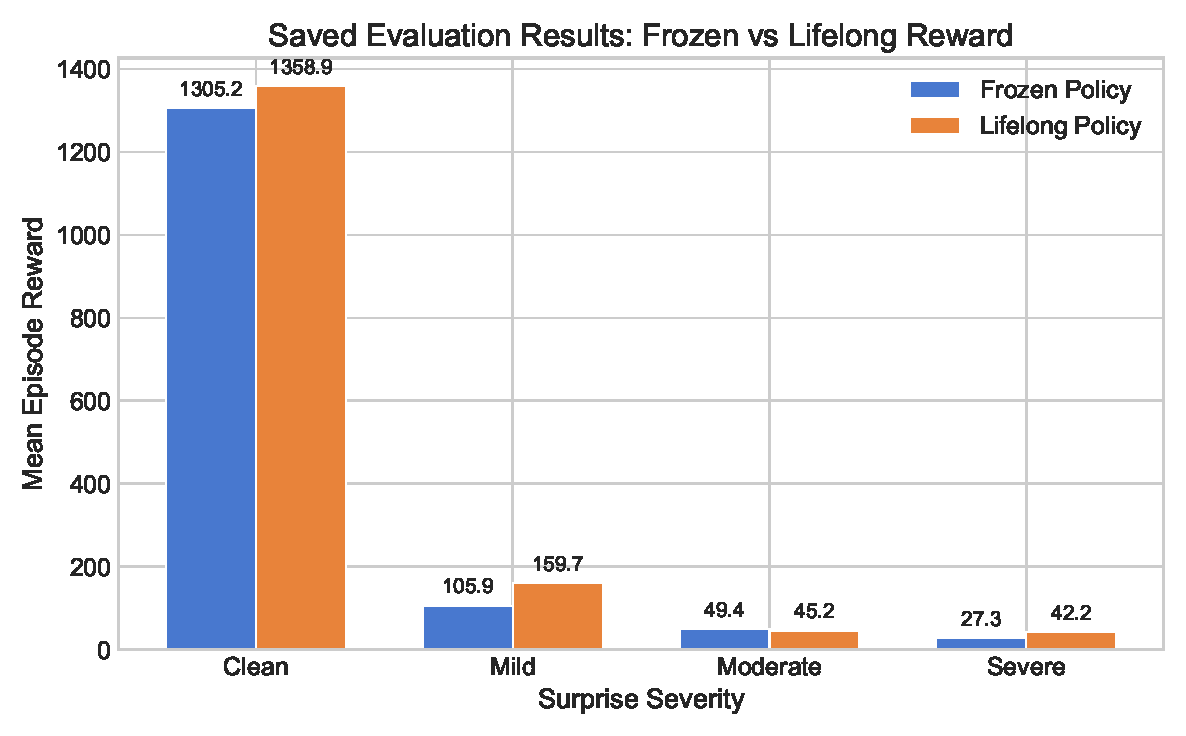
\includegraphics[width=0.82\linewidth]{fig1_frozen_vs_lifelong.pdf}
  \caption{Frozen versus lifelong mean reward across surprise severity. The saved single-seed result shows gains on clean, mild, and severe, with a moderate-severity regression.}
  \label{fig:frozen-vs-lifelong}
\end{figure}

\subsection{Forgetting and ablations}

The forgetting probe adapts on severe and then evaluates on clean. Clean reward is 1308.9 before adaptation and 1386.1 after adaptation, so the evaluator reports \texttt{forgetting\_detected: false}. This supports the retention claim for the saved seed, though not a multi-seed guarantee.

The ablation run evaluates severe surprise with 15 episodes per variant. Removing individual safeguards can increase mean reward but also increases variance. The full method has lower variance, suggesting a stability-performance tradeoff.

\begin{figure}[t]
  \centering
  
\includegraphics[width=0.82\linewidth]{fig3_ablations.pdf}
  \caption{Ablation results under severe surprise. Ablated variants can produce higher means but with substantially higher variance than the full method.}
  \label{fig:ablations}
\end{figure}

\subsection{Sequential continual-learning matrix}

The per-severity evaluator resets from the baseline for each severity. To directly test continual learning, we also run one sequence: clean, mild, moderate, severe. After each phase, the same lifelong policy is evaluated on every severity, producing a matrix $R[i,j]$ where row $i$ is the completed adaptation phase and column $j$ is the evaluation task. The matrix supports backward-transfer, forward-transfer, and remembering metrics commonly used in continual-learning diagnostics \citep{lopezpaz2017gradient,van2024continual}.

\begin{table}[t]
  \centering
  \caption{Sequential continual-learning matrix for the lifelong policy. Rows are completed adaptation phases; columns are evaluation tasks.}
  \label{tab:continual-matrix}
  \begin{tabular}{lrrrr}
    \toprule
    Phase completed & Clean & Mild & Moderate & Severe \\
    \midrule
    after clean & 1316.0 & 146.9 & 48.1 & 38.5 \\
    after mild & 1261.3 & 143.5 & 94.9 & 21.5 \\
    after moderate & 1406.2 & 159.2 & 40.3 & 31.8 \\
    after severe & 1322.9 & 131.2 & 92.0 & 26.1 \\
    \bottomrule
  \end{tabular}
\end{table}

\begin{figure}[t]
  \centering
  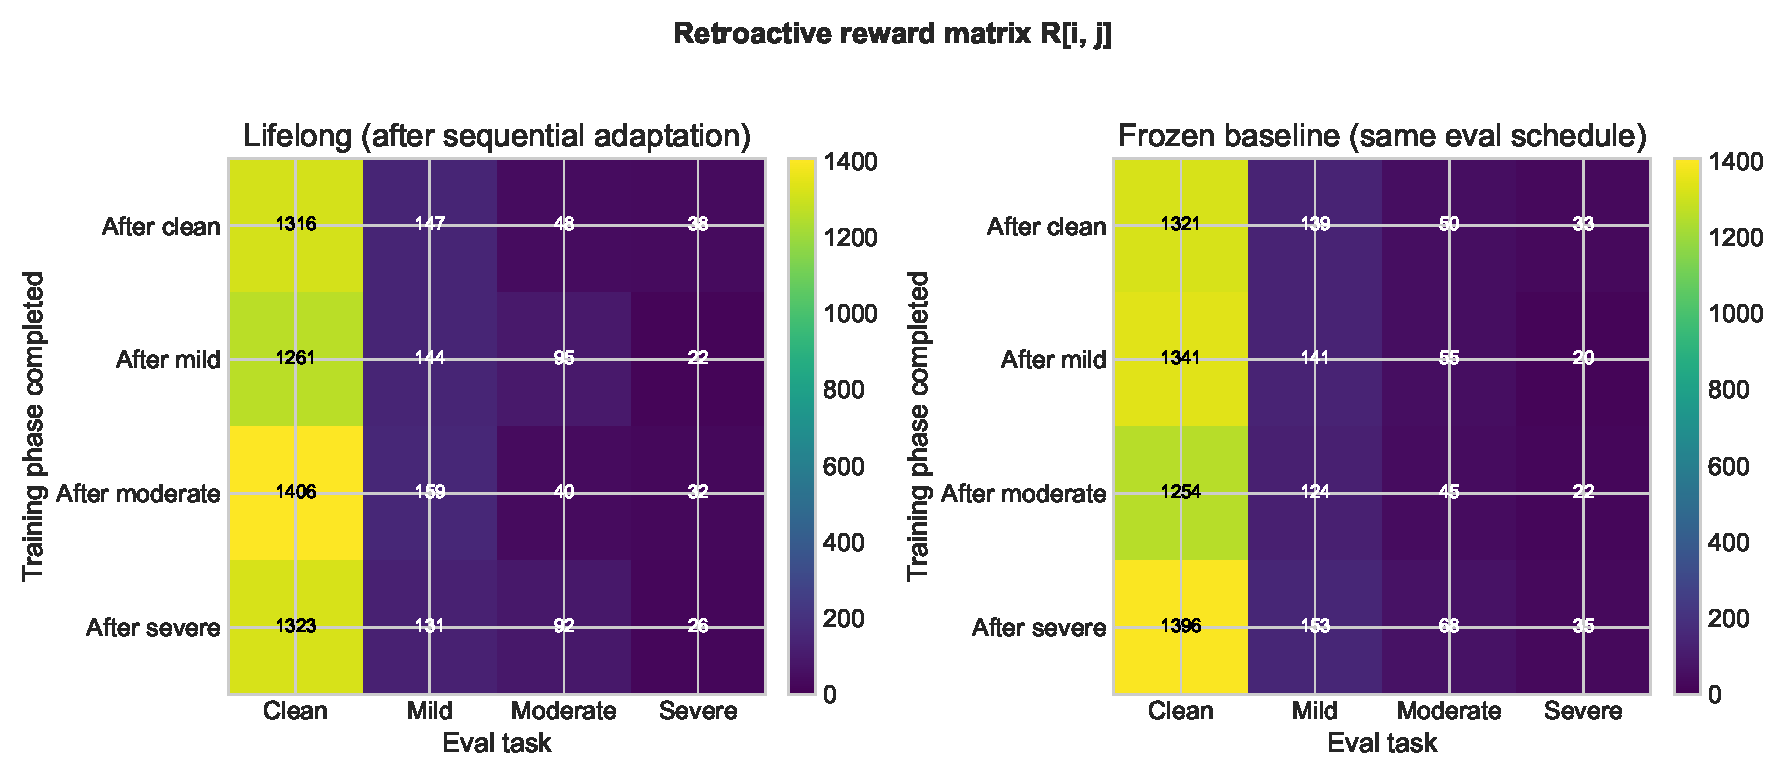
\includegraphics[width=0.90\linewidth]{fig6_continual_matrix.pdf}
  \caption{Retroactive reward matrices for lifelong and frozen policies. The clean column shows that clean performance is explicitly re-tested after later adaptation phases.}
  \label{fig:continual-matrix}
\end{figure}

The clean column remains in the same range across the sequence: 1316.0, 1261.3, 1406.2, and 1322.9. The final average reward is 393.1 for lifelong versus 412.9 for the frozen reference, while backward transfer is +15.4, forward transfer is +17.2, and remembering is 1.0. This is evidence of clean retention and positive transfer metrics, not evidence that lifelong adaptation dominates frozen performance on every metric.

\section{Discussion and limitations}

The results show that post-training surprises are damaging for the clean-trained policy. The lifelong method recovers some reward under mild and severe surprise and retains clean performance in the forgetting and sequential probes. The moderate result is mixed, and the final continual average reward is lower than the frozen reference. The honest interpretation is that the project demonstrates a working retention-oriented adaptation pipeline, but the current trigger and objective are not strong enough for universal robustness.

Several limitations matter. All canonical results use one seed, so statistical confidence is limited. The swarm has only two drones. Severe absolute reward remains low. The confidence trigger is conservative, with a 2\% adaptation rate in the main per-severity run. The simulator is simplified, and the method adapts only between episodes. These constraints limit claims about real-world robustness and scaling.

\section{Author contributions}

\textbf{TODO\_AUTHOR\_CONTRIBUTIONS:} Replace this paragraph before submission with the verified division of work among Tanush Vijayakumar Savadi, Deveshi Singh, and Ron Kleinhause-Goldman. The course instructions explicitly require communicating who worked on which parts of the project. A suitable format is: environment and surprise suite; PPO baseline and training; confidence monitor and lifelong adaptation; continual-learning evaluation; plots, report, and presentation.

\section{Conclusion}

We built and evaluated a confidence-triggered lifelong adaptation system for drone swarms under post-training surprises. The system combines a clean-trained shared PPO policy, a controlled surprise suite, confidence-triggered between-episode updates, and anti-forgetting safeguards. The saved results show partial robustness and clean retention in a single-seed setting. The next steps are multi-seed validation, stronger adaptation objectives, larger swarms, richer surprises, and peer-help mechanisms.

\bibliographystyle{plainnat}
\bibliography{references}

\end{document}
